\chapter{Аналитическая часть}

В этом разделе будут представлены описания алгоритмов сортировки пирамидальная,
блинная, перемешиванием.

\section{Пирамидальная сортировка}

Пирамида (англ. binary heap) определяется как структура данных, представляющая собой объект-массив, который можно рассматривать как почти полное бинарное дерево. Каждый узел этого дерева соответствует определенному элементу массива. На всех уровнях, кроме, может быть, последнего, дерево полностью заполнено (заполненным считается уровень, который содержит максимально возможное количество узлов). Последний уровень заполняется слева направо до тех пор, пока в массиве не закончатся элементы. 

В пирамиде, представленной на рисунке \ref{fig:heap_structs}, число в окружности, представляющей каждый узел дерева, является значением, сортируемым в данном узле. Число над узлом — это соответствующий индекс массива. Линии, попарно соединяющие элементы массива, обозначают взаимосвязь вида “родитель-потомок”. Родительские элементы всегда расположены слева от дочерних. Данное дерево имеет высоту, равную 3; узел с индексом 4 (и значением 8) расположен на первом уровне.

\begin{figure}[h]
	\centering
	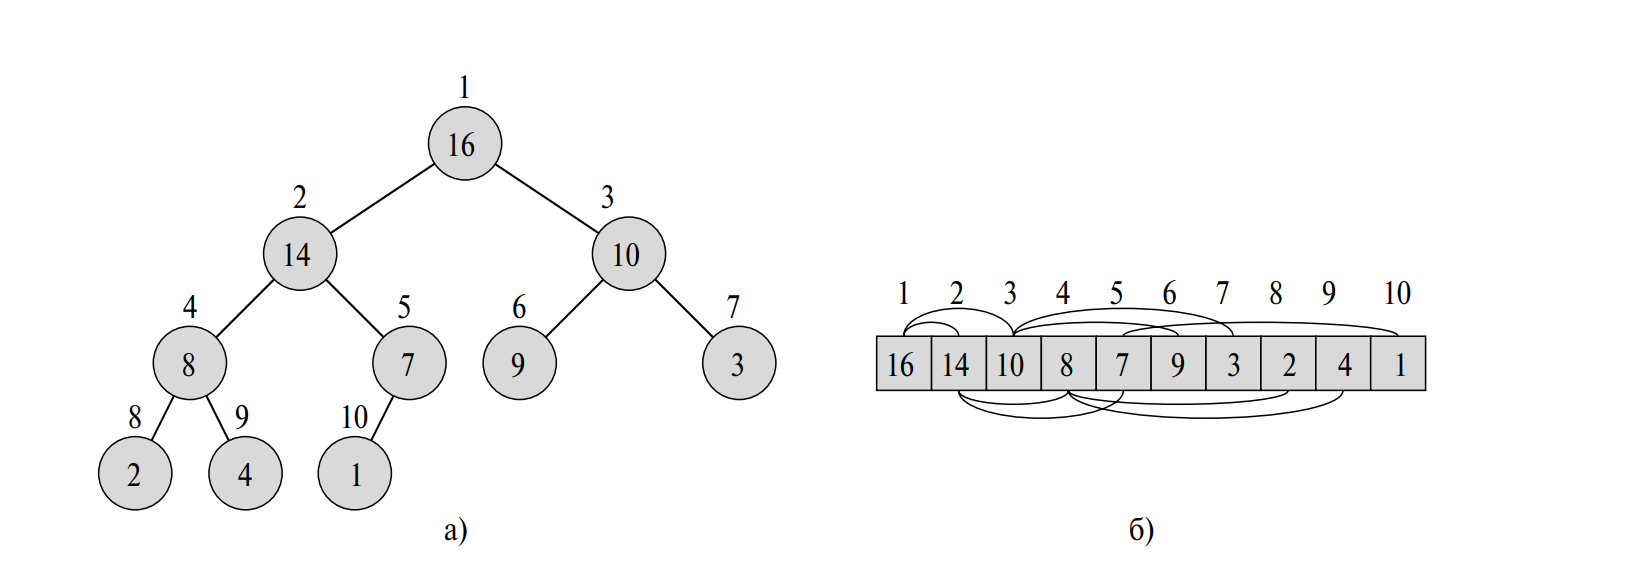
\includegraphics[height=0.25\textheight]{img/heap_structs.jpg}
	\caption{Пирамида, представленная в виде a) бинарного дерева и б) массива}
	\label{fig:heap_structs}
\end{figure}

Обозначим, что:
\begin{enumerate} 
	\item Родительский элемент в массиве будет находится под индексом - $\frac{i}{2}$;
	\item Правый потомок в массиве будет находится под индексом - $2 \cdot i$;
	\item Левый потомок в массиве будет находится под индексом - $2 \cdot i + 1$.
\end{enumerate}

Различают два вида бинарных пирамид: неубывающие и невозрастающие. В пирамидах обоих видов значения, расположенные в узлах, удовлетворяют свойству пирамиды (heap property), являющемуся отличительной чертой пирамиды того или иного вида. Свойство невозрастающих пирамид (max-heap property) заключается в том, что для каждого отличного от корневого узла с индексом $i$ выполняется следующее неравенство

\begin{equation}
	A[i / 2] \geq A[i]
\end{equation}

Другими словами, значение узла не превышает значение родительского по отношению к нему узла. Таким образом, в невозрастающей пирамиде самый большой элемент находится в корне дерева, а значения узлов поддерева, берущего начало в каком-то элементе, не превышают значения самого этого элемента. Принцип организации неубывающей пирамиды (min-heap) прямо противоположный. Свойство неубывающих пирамид (min-heap property) заключается в том, что для всех отличных от корневого узлов с индексом $i$ выполняется такое неравенство:

\begin{equation}
	A[i / 2] \leq A[i]
\end{equation}

Таким образом, наименьший элемент такой пирамиды находится в ее корне.

\section{Сортировка перемешиванием}
\textbf{Алгоритм сортировки перемешиванем} является модификацией алгоритма
сортировки пузырьком. В отличие от сортировки пузырьком, где происходит обход
последовательности только в одном направлении, в алгоритме сортировки
перемешиванием после достижения одной из границ рабочей части
последовательности (то есть той части, которая еще не отсортирована и в которой
происходит смена элементов) меняет направление движения. При этом при движении
в одном направлении алгоритм перемещает к границе рабочей области максимальный
элемент, а в другом направлении -- минимальный элемент. Границы рабочей части
последовательности устанавливаются в месте последнего обмена. 

\section{Блинная сортировка}
\textbf{Блинная сортировка (pancake sort)} – алгоритм сортировки массива, в котором сортировка осуществляется переворотом части массива.

В этом алгоритме, к массиву, позволено применять только одну операцию – переворот части массива. И в отличии от других методов сортировки, где пытаются уменьшить количество сравнений, в этом нужно минимизировать количество переворотов.

Идея алгоритма заключается в том, чтобы за каждый проход, переместить максимальный элемент в конец массива.

\section*{Вывод}

В данной работе необходимо реализовать алгоритмы сортировки, описанные в данном разделе, 
а также провести их теоритическую оценку и проверить ее экспериментально.
